\section{APX-completeness for segments parallel to axis}
\label{section:segment_apx}

In this section we analyze if there exists an
$(1+\epsilon)$-approximation
scheme for set cover with rectangles.
We will show that we can restrict this problem
to a very easy setting:
segments parallel to axes and allow (1/2)-extension,
and the problem is still APX-hard.
Note that segments are just degenerated rectangles
with one side being very narrow.


Our results can be summarized in the following
theorem and this section aims to prove it.

\begin{tw}{
\label{segment_cover_apx_hard}
	\textbf{(axis-parallel segment set cover with 1/2-extension is APX-hard)}.	
	Unweighted geometric set cover
	with axis-parallel segments in 2D (even with 1/2-extension)
	is APX-hard,
	i.e. assuming $P\neq NP$, there does not exist a PTAS
	for this problem.
}\end{tw}
 
Theorem \ref{segment_cover_apx_hard} implies the following.

\begin{corollary}{
\label{rectangle_cover_apx_hard}
	\textbf{(rectangle set cover is APX-hard)}.	
	Unweighted geometric set cover
	with rectangles (even with 1/2-extension) is APX-hard.
}\end{corollary}


We will prove Theorem \ref{segment_cover_apx_hard}
by taking a problem that is APX-hard
and showing a reduction.
For this problem we choose
MAX-(3,3)-SAT which we define in detail below.

Given an instance $I$ of MAX-(3,3)-SAT,
we will construct an instance $J$ of 
axis-parallel segment set cover problem,
such that an $(1+c\cdot\epsilon)$-approximation for $J$
will yield a $(1+\epsilon)$-approximation for $I$,
for any constant $c > 1$.
Therefore if there would exist a PTAS for
the axis-parallel segment set cover problem,
we would produce a PTAS for MAX-(3,3)-SAT, which 
does not exist assuming $P\neq NP$.


\subsection{MAX-(3,3)-SAT problem}
\begin{defi}
\textbf{MAX-3SAT} is an optimization problem. We are given a 3-CNF
formula, and need to find an assignment of variables
that satisfies the most clauses.
\end{defi}

\begin{defi}
\textbf{MAX-(3,3)-SAT} is a MAX-3SAT with an additional
restriction that every variable appears in exactly 3 clauses,
so that the number of clauses is equal to number of variables.
\end{defi}

In the lemmas above we use
a property of MAX-(3,3)-SAT proved in \cite{hastad} and described in
Theorem \ref{hastadtheorem}.

\begin{tw}{
	\label{hastadtheorem}
	\textbf{\cite{hastad}}
	
	For any $\epsilon > 0$, it is NP-hard to distinguish satisfiable
	(3,3)-SAT formulas from
	%This broke x-satisfiable to next line
	\linebreak\mbox{$(7/8 + \epsilon)$-satisfiable}
	(3,3)-SAT formulas. Said equivalently, MAX-(3,3)-SAT
	is nonapproximable beyond the random assignment threshold
	on satisfiable instances.
}\end{tw}

The following lemma encapsulates the properties
of the reduction described in this section,
and it allows to prove Theorem \ref{segment_cover_apx_hard}.

\begin{lemma}{
	\label{apxconstruction}
	Given an instance $S$ of  MAX-(3,3)-SAT 
	with $n$ variables and optimal result~$OPT(S)$,
	we can construct an instance $I$ of axis-parallel segments in 2D
	with $\delta$-extensions, such that:
	\begin{enumerate}
	\item for every solution $X$ of problem $I$,
	there exists a solution of $S$ of size at least  $15n - |X|$;
	
	\item for every solution $X$ of problem $S$,
	there exists a solution of $I$ of size $15n - |X|$;
	
	Therefore optimal solution of $I$ is $OPT(I) = 15n - OPT(S)$. 
	\end{enumerate}
	
}\end{lemma}

We prove Lemma \ref{apxconstruction} in
subsequent sections, but meanwhile let's prove
Theorem \ref{segment_cover_apx_hard} using Lemma \ref{apxconstruction}
and Theorem \ref{hastadtheorem}.

\paragraph{Proof of Theorem \ref{segment_cover_apx_hard}}
Take any $0 < \epsilon < 1/(15 \cdot 8)$.

Let's assume that there exists an $(1+\epsilon)$-approximation scheme
for unweighted geometric set cover with axis-pararell segments in 2D
with (1/2)-extensions.
We will construct an algorithm distinguishing instances of
MAX-(3,3)-SAT
in Theorem \ref{hastadtheorem}.

Take an instance~$S$ of MAX-(3,3)-SAT to be distinguished
and construct an instance of geometric set cover $I$
using Lemma \ref{apxconstruction}.

We now use the $(1+\epsilon)$-approximation scheme
for instances of geometric set cover on $I$,
denote the cost of the result of this approximation as $approx(I)$.

We will prove that 
if $approx(I) \ge 15n - (\frac{7}{8} + \epsilon)n$ then $S$
satisfied at most $(\frac{7}{8}+\epsilon)n$ clauses,
and if $approx(I) < 15n - (\frac{7}{8} + \epsilon)n$ then $S$ was
satisfiable.

\subparagraph{Assume $S$ satisfiable}
From the definition of $S$ being satisfiable, we have:
$$OPT(S) = n$$

From Lemmma \ref{apxconstruction} we have:

$$OPT(I) = 14n$$

$$approx(I) \le (1+\epsilon)OPT(I) = 14n(1+\epsilon)
	= 14n + 14\epsilon\cdot n =$$ 
	$$= 14n + (15\epsilon - \epsilon)n < 
  14n + \left(\frac{1}{8} - \epsilon\right)n 
= 15n - \left(\frac{7}{8} + \epsilon\right)n$$

\subparagraph{Assume $S$ at most
$\left(\frac{7}{8} + \epsilon\right)n$ satisfiable}
From defintion of $S$ being at most 
$\left(\frac{7}{8} + \epsilon\right)n$ satisfiable, we have:
$$OPT(S) \le \left(\frac{7}{8} + \epsilon\right)n$$

From Lemmma \ref{apxconstruction} we have:
$$OPT(I) = 15n - \left(\frac{7}{8} + \epsilon\right)n$$

$$approx(I) \ge OPT(I) = 15n - \left(\frac{7}{8} + \epsilon\right)n$$


Therefore, by using the assumed to exist $(1+\epsilon)$-approximation
scheme for segment set cover,
it is possible to distinguish $S$ from
being satisfiable and at most $(\frac{7}{8} + \epsilon)n$ satisfiable,
since there exists a threshold on the
approximation result in segment set cover that distinguishes
these two cases.
This is a contradiction, hence the approximation scheme cannot exist.

\subsection{Reduction construction}
We will show reduction from MAX-(3,3)-SAT problem
to geometric set cover with segments
parallel to axis. Moreover the instance
of geometric set cover will be robust
to 1/2-extensions (have the same optimal solution
after 1/2-extension).

The construction will be composed of 2 types of gadgets:
\textbf{VARIABLE-gadgets} and \textbf{CLAUSE-gadgets}.
CLAUSE-gadgets would be constructed using two \textbf{OR-gadgets}
connected together.


\subsubsection{VARIABLE-gadget}

VARIABLE-gadget is responsible for choosing a value of variable
in CNF formula. It allows two minimal solution
and every minimal solution must use exactly one of the $a$ and $b$
segments, so you can assign  a binary value to the variable.

\paragraph{Points.}

Define points:
\begin{figure}[h]
\centering
\def\svgwidth{0.5\columnwidth}
\input{apx_choose_variable.pdf_tex}
\caption{\textbf{Choose variable value gadget.}
We denote set of points marked with black circle as $C\_variable_i$
and need to be covered (are part of set $\points$).
We denote set of red segments as $x^{false}_i$
and set of blue segments as $x^{true}_i$.}
\label{fig:apx_choose_variable}
\end{figure}

TODO: inline $L = 12n$ after finishing these formulas

\begin{center}
\begin{tabular}{ l l l l}
	$a_{i} = (-L, 4i)$ &
	$b_{i} = (-\frac{2}{3}L, 4i)$ & 
	$c_{i} = (-\frac{1}{3}L, 4i)$ & 
	$d_{i} = (-L, 4i+1)$ \\  
	$e_{i} = (-\frac{2}{3}L, 4i+1)$ & 
	$f_{i} = (-\frac{2}{3}L, 4i+2)$ &
	$g_i = (L, 4i)$ &
	$h_i = (L, 4i+2)$
\end{tabular}
\end{center}

Let's define $$C\_variable_i =  \{a_i, b_i, c_i, d_i, e_i, f_i\}$$	


\paragraph{Segments.}

Let's define 

$$x^{true}_i =\{ (a_i, d_i), (b_i, f_i), (c_i, g_i)\}$$
$$x^{false}_i = \{(a_i, c_i), (d_i, e_i), (f_i, h_i)\}$$

$$P\_variable_i = x^{true}_i \cup x^{false}_i$$


\begin{lemma}
\label{choose_variables_solution}
For any $1 \le i \le n$, points $C\_variable_i$
can be covered using 3 segments from $P\_variable_i$.
\end{lemma}

\paragraph{Proof.}
We can use either set $x^{true}_i$ or $x^{false}_i$.


\begin{lemma}
\label{choose_variables_no_less}
For any $1 \le i \le n$, points $C\_variable_i$
can not be covered with less than 3 segments from $P\_variable_i$.
\end{lemma}

\paragraph{Proof.}
There is independent set $\{d_i, f_i, c_i\}$ of size 3, therefore it can
not be covered with less than 3 sets (segments).


\begin{lemma}
\label{choose_variables_both}
If both segments $\xTrueSegment$ and $\xFalseSegment$ are chosen, then
the covering the remaining points from $C\_variable_i$
requires at least 2 different
segments from $P\_variable_i$.
\end{lemma}
\paragraph{Proof.}
There is an independent set $\{a_i, e_i\}$ of size 2
in $C\_variable_i$ - $\{c, f, g, h\}$,
therefore it can not be covered with less than 2 sets (segments).


\subsubsection{OR-gadget}

OR-gadget has 3 important segments
-- $x, y, result$. $x$ and $y$ don't count to the weight of solution
of OR-gadget (they are part of different gadgets).
It has a minimal solution of weight $w$
and $result$ can be chosen only if $x$ or $y$ are also chosen
for the solution.
If none of them are chosen, then solution
choosing $result$ segment has weight at least $w+1$.
Therefore the following formula holds for a solution $R$
assuming that $R$ uses only $w$ from this OR-gadget:

$$ (x \in R) \lor (y \in R) \iff result \in R  $$

\paragraph{Points.}

\begin{figure}[h]
\centering
\def\svgwidth{0.5\columnwidth}
\input{apx_or_gadget.pdf_tex}
\caption{
\textbf{OR-gadget.} We denote these point as $or\_gadget_{i, j}$. 
We denote set of red segments as $or^{false}_{i, j}$,
set of blue segments as $or^{true}_{i, j}$,
green and yellow segments as $or\_move\_variable_{i, j}$.
}
\label{fig:apx_or_gadget}
\end{figure}

	\begin{center}
\begin{tabular}{ l l l l}

	$l_0 = (0, 0)$ &
	$m_0 = (0, 1)$ &
	$n_0 = (0, 2)$ &
	$o_0 = (0, 3)$ \\
	$p_0 = (0, 4)$ &
	$q_0 = (1, 1)$ &
	$r_0 = (1, 3)$ &
	$s_0 = (2, 1)$ \\
	$t_0 = (2, 2)$ &
	$u_0 = (2, 3)$ &
	$v_0 = (3, 2)$ &
\end{tabular}
\end{center}


	$$vec_{i, j} = (10i + 3 + 3j, 4n + 2j)$$
	
	Define 
	$\{ l_{i, j}, m_{i, j} \ldots v_{i, j} \}$
	as $\{l_0, m_0 \ldots v_0\}$ shifted by $vec_{i, j}$

Note that $v_{i, 0} = l_{i, 1}$ (see Figure~\ref{fig:apx_clause})
 
  $$C\_or\_gadget_{i, j} = 
 \{l_{i, j}, m_{i, j}, n_{i, j}, o_{i, j},
 p_{i, j}, q_{i, j}, r_{i, j}, s_{i, j}, t_{i, j}, u_{i, j} \}
 $$
 
\paragraph{Segments.}

We define names subsets of segments, to refer to them in lemmas.
 
$$or^{false}_{i, j} =
\{ (q_{i, j}, r_{i, j}), (s_{i, j}, u_{i, j})\}$$
$$or^{true}_{i, j} =
\{ (m_{i, j}, s_{i, j}), (o_{i, j}, u_{i, j}),
(t_{i, j}, v_{i, j}) \}$$

$$or\_move\_variable_{i, j} =
\{ (l_{i, j}, n_{i, j}), (n_{i, j}, p_{i, j})\}$$

Segments in OR-gadget:

$$P\_or\_gadget_{i, j} = 
  or^{false}_{i, j} \cup or^{true}_{i, j} \cup or\_move\_variable_{i, j}
  $$


\begin{lemma}
\label{cover_or_true}
For any $1 \le i \le n, j \in \{0, 1\}$ and 
 $x \in \{l_{i, j}, p_{i, j}\}$ we can cover points in
$C\_or\_gadget_{i, j} - \{ x\} \cup \{v_{i, j}\}$
with 4 segments.
\end{lemma}

\paragraph{Proof.}
We can do that using one segment from
$or\_move\_variable_{i, j}$
(chosen depending on the value of $x$)
and all segments from $or^{true}_{i, j}$.

\begin{lemma}
\label{cover_or_false}
For any $1 \le i \le n, j \in \{0, 1\}$, we can cover points in
$C\_or\_gadget_{i, j}$ with 4 segments from $P\_or\_gadget_{i,j}$.
\end{lemma}
\paragraph{Proof.}
We can do that using  $or\_move\_variable_{i, j}$
and $or^{false}_{i, j}$.


\subsubsection{CLAUSE-gadget}


CLAUSE-gadget is responsible for calculating if choice of the
variable values meets the clause in formula.
It has minimal solution of weight $w$ if at least one variable
in the clause has a correct value.
Otherwise it has minimal solution $w+1$.
This way by the minimal solution for the whole problem, we can tell
how many clauses were satisfiable.

The CLAUSE-gadgets consist of two OR-gadgets.
We don't want the CLAUSE-gadgets to be crammed 
somewhere between
the very long variable segments. That's why we have a simple
gadget to \textit{pass} the value of the segment, ie. segments
$(x_{i, 0}, x_{i, 1}), (y_{i, 0}, y_{i, 1}), (z_{i, 0}, z_{i, 1})$.
Two segments and one of them is chosen if $x$ was chosen
in the solution and the other one if $x$ wasn't.

\paragraph{Points.}


\begin{figure}[h]
\centering
\def\svgwidth{0.8\columnwidth}
\input{apx_clause.pdf_tex}
\caption{\textbf{CLAUSE-gadget.}
We denote set of these points as $C\_clause_i$.
Every green rectangle is an OR-gadget.
$y$-coordinates of $x_{i, 0}$, $y_{i, 0}$ and $z_{i,0}$
depend on the values of variables in the $i$-th clause.
}
\label{fig:apx_clause}
\end{figure}

TODO: Rephrase it

Assuming clause $C_i = x_i \lor y_i \lor z_i$,
function $idx(w)$ is returning index of the variable $w$,
function $neg(w)$ is returning whether variable $w$ is negated
in a clause.

\begin{center}
\begin{tabular}{ l l }
	$x_{i, 0} = (10i+1, 4\cdot idx(x_i) + 2\cdot neg(x_i))$ &
	$x_{i, 1} = (10i+1, 4n)$ \\
	$y_{i, 0} = (10i+2, 4\cdot idx(y_i) + 2\cdot neg(y_i))$ &
	$y_{i, 1} = (10i+2, 4n + 4)$ \\
	$z_{i, 0} = (10i+3, 4\cdot idx(z_i) + 2\cdot neg(z_i))$ &
	$z_{i, 1} = (10i+3, 4n + 6)$
\end{tabular}
\end{center}
	
 
 $$move\_variable_i = 
 \{x_{i, j} : j \in \{0, 1\}\} \cup
 \{y_{i, j} : j \in \{0, 1\}\} \cup
 \{z_{i, j} : j \in \{0, 1\}\} 
 $$
 
 $$C\_clause_i = 
 move\_variable_i \cup C\_or\_gadget_{i, 0}
 \cup C\_or\_gadget_{i, 1} \cup \{v_{i, 1} \} 
 $$

\paragraph{Segments.}

\begin{eqnarray*}
P\_clause_i & = & \{ (x_{i, 0}, x_{i, 1}),
(y_{i, 0}, y_{i, 1}),
(z_{i, 0}, z_{i, 1}),
(x_{i, 1}, l_{i, 0}),
(y_{i, 1}, p_{i, 0}),
(z_{i, 1}, p_{i, 1}),
\} \cup \\
& & \cup \ P\_or\_gadget_{i, 0} \cup P\_or\_gadget_{i, 1}
\end{eqnarray*}

\begin{lemma}
\label{cover_clauses_solution_true}
For any $1 \le i \le n$ and $a \in \{ x_{i, 0}, y_{i, 0}, z_{i, 0}\}$,
points $C\_clause_i - \{a\}$ can be covered using 11 segments
from $P\_clause_i$.
\end{lemma}

\paragraph{Proof.}
For $a = x_{i, 0}$ (analogous proof for $y_{i, 0}$):
First we use Lemma~\ref{cover_or_true} twice with excluded $x = l_{i, 0}$ and
$x = l_{i, 1} = v_{i, 0}$,
resulting with 8 segments $or^{true}_{i, 0} \cup or^{true}_{i, 1}$
which cover all required points apart from
$x_{i, 1}, y_{i, 0}, y_{i, 1}, z_{i, 0}, z_{i, 1}, l_{i, 0}$.
We cover those using additional 3 segments:
$\{ (x_{i, 1}, l_{i, 0}), (y_{i, 0}, y_{i, 1}),
(z_{i, 0}, z_{i, 1}) \}$

For $a = z_{0, i}$:
Using Lemma~\ref{cover_or_false} and Lemma~\ref{cover_or_true} with
$x = p_{i, 1}$,
resulting with 8 segments $or^{false}_{i, 0} \cup or^{true}_{i, 1}$
which cover all required points apart from
$x_{i, 0}, x_{i, 1}, y_{i, 0}, y_{i, 1}, z_{i, 1}, p_{i, 1}$.
We cover those using additional 3 segments:
$\{ (x_{i, 0}, x_{i, 1}), (y_{i, 0}, y_{i, 1}),
(z_{i, 1}, p_{i, 1}) \}$.

\begin{lemma}
\label{cover_clauses_solution_false}
 Points $C\_clause_i$ can be covered with 12 segments from $P\_clause_i$.
\end{lemma}

\paragraph{Proof.}
Using Lemma \ref{cover_or_false} twice we can
cover $or\_gadget_{i,0}$ and  $or\_gadget_{i,1}$
with 8 segments.

To cover the remaining points we additionally use:
$\{ (x_{i, 0}, x_{i, 1}), (y_{i, 0}, y_{i, 1}),
(z_{i, 0}, z_{i, 1}), (t_{i, 1}, v_{i, 1}) \}$


\begin{lemma}
\label{cover_clauses_segments_no_less}
For any $1 \le i \le n$,
points $C\_clause_i - \{ x_{i, 0}, y_{i, 0}, z_{i, 0}\}$
can not be covered using less than 11 segments from $P\_clause_i$.

All points $C\_clause_i$ can not be covered with less than 12 segments
from $P\_clause_i$.
\end{lemma}


\paragraph{Proof of no cover with less than 12 segments.}
There is independent set of 12 points in $C\_clause_i \supseteq
\{ x_{i, 0}, y_{i, 0}, z_{i, 0}, l_{i, 0}, p_{i, 0}, q_{i, 0},
u_{i, 0}, v_{i, 0} = l_{i, 1}, p_{i, 1}, q_{i, 1}, u_{i, 1}, v_{i, 1} \}$.

\paragraph{Proof of no cover with less than 11 segments.}

We can choose disjoint sets $X, Y, Z$ such that
$X \cup Y \cup Z \subseteq C\_clause_i - \{x_{i, 0}, y_{i, 0}, z_{i, 0}\}$
and there are no segments covering points from different sets.
And we will prove lower bounds for each of these sets.

$$X = \{x_{i, 1}, y_{i, 1}, z_{i, 1}\}$$

Set $X$ is an indendent set, so it must be covered with 3 segments.

$$Y = or\_gadget_{i, 0} - \{l_{i, 0}, p_{i, 0}\}$$
$$Z = or\_gadget_{i, 1} - \{l_{i, 1}, p_{i, 1}\}$$


For both $Y$ and $Z$ we can check all of the subsets of 3 segments
with brutforce that none of them cover, so they have to be covered with
4 segments.

TODO: Funny fact, neither Y nor Z doesn't have independent set of size 4.

Therefore $C\_clause_i$ must be covered with at least 3 + 4 + 4 = 11 segments.

\subsubsection{Summary}

Add some smart lemmas that sets will be exclusive to each other.

\begin{lemma}
\textbf{Robustness to 1/2-extensions}. For every segment $s \in \sets$,
$s$ and $s^{+1/2}$ cover the same points from $\points$.
\end{lemma}


\subsection{Summary of contruction}

\begin{figure}
\centering
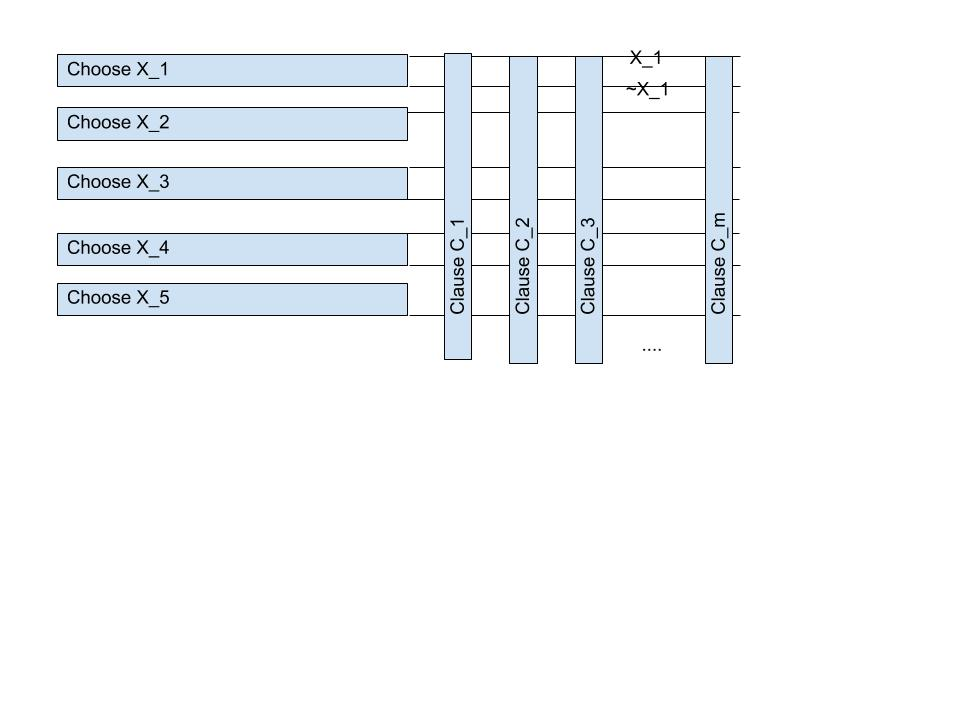
\includegraphics[width=\linewidth]{segment_apx_sketch.jpg}
\caption{\textbf{General schema.}}
General layout of VARIABLE-gadget and CLAUSE-gadget and how they
interact with each other.

TODO: Rename Choose X to VARIABLE-gadget and Clause C to CLAUSE-gadget.
\label{fig:segment_apx_sketch}
\end{figure}

We define:
$$\points := \bigcup_{1 \le i \le n} C\_variable_i \cup C\_clause_i $$
$$\sets := \bigcup_{1 \le i \le n} P\_variable_i \cup P\_clause_i $$

The subsequent sections define these sets.

We will prove some properties of different gadgets.
Every segment for a gadget will only cover points 
in this gadget (won't interact with any diferent gadget),
so we can prove lemmas \textit{locally}.


TODO: $y$ axis is increasing values downward on figures
(not upwards like in normal).

\subsection{Proofs of construction Lemma \ref{apxconstruction}}
\begin{lemma}
	\label{construction_correctness}
	Given an instance of MAX-(3,3)-SAT of size $n$
	with optimal solution $k$.
	For instance of geometric cover, constructed
	according to Lemma~\ref{apxconstruction}, 
	there exists a solution of weight $15n - k$.
\end{lemma}
\paragraph{Proof.}
Let's name the assignments of the variables in MAX-(3,3)-SAT instance,
that achieve the optimal solution,
$y_1$,~$y_2$~$\ldots$~$y_n$,
Let's cover every VARIABLE-gadget with solution described in
Lemma~\ref{choose_variables_solution},
in the $i$-th gadget choosing the set of segments responsible for the
value of $y_i$
(true -- $x_i^{true}$ or false -- $x_i^{false}$).

Cover every satisfied CLAUSE-gadget with solution described in
Lemma~\ref{cover_clauses_solution_true}
and unsatisfied CLAUSE-gadget with solution from
Lemma~\ref{cover_clauses_solution_false}.

This solution uses $3n + (11m + (m-k)) = 15n - k$ segments.

\begin{lemma}
	\label{construction_completness}
	Given an instance of MAX-(3,3)-SAT of size $n$,
	and solution of size $w$ to the instance of geometric cover,
	constructed	according to Lemma~\ref{apxconstruction},  
	there exists a solution to MAX-(3,3)-SAT of size at least $15n - w$.
\end{lemma}
\paragraph{Proof.}
Among $x_i^{true} \cup x_i^{false}$,
we need to use at least 3 segments (Lemma~\ref{choose_variables_no_less}).
If we have chosen both segments $\xTrueSegment$ and $\xFalseSegment$,
then we have used at least 4 segments (Lemma~\ref{choose_variables_both}).

If we chose at most one of the segments $\xTrueSegment$ and $\xFalseSegment$,
choose the corresponding variable value to the solution.
If we chose both segments,
choose the value that appears in most (at least 2) clauses.
If we have chosen none of the segments, choose any value.

To cover $\bigcup_{1 \le i \le n} C\_variable_i$
we have used at least $3n + a$ segments,
where $a$ is the number of $i$ such that we have chosen both
values $\xTrueSegment$ and $\xFalseSegment$.

Among the segments responsible for the clause $C_i = x \lor y \lor z$
we need to use at least 11 segments
(Lemma~\ref{cover_clauses_segments_no_less})
and if we can cover it with 11 segments, then we have 
earlier chosen
segment responsible for the value of variable $x$, $y$ or $z$
that satisfies $C_i$.

So we have at least 11 segments for satisfied clauses
and at least 12 segments
for unsatisfied clauses, so we cover it with 
at least $11n + b$ segments, where $b$ is number of clauses
where none of the variables $x, y, z$ were chosen.
If the segment responsible for value of $x$ was taken,
but this variable is set to have different value,
then we have chosen segments for both $x$ and $\neg x$ for this variable,
so "we cheated" and this maybe clause is not met,
but we assigned the value for this $x_i$ that meets
the most clauses, so for each of such "cheated" variables,
at most one of the clauses isn't met.

So there are at most $a+b$ unsatsfied clauses in this instance,
so we have shown the assignment with at least  $n-(a+b)$ satisfied clauses.

$$w \ge 3n + a + 11n + b = 14n + a + b$$
$$15n - w  \le 15n - 14 n - a - b = n - (a+b)$$

\subsubsection{Proof of Lemma \ref{apxconstruction}}
Given an instance of MAX-(3,3)-SAT of size $n$
with optimal result $k$.
Let's construct an instance of geometric cover,
constructed in aforementioned manner.

Given the Lemma~\ref{construction_correctness}, we know
the optimal solution for the constructed geometric cover is
at most $15n - k$ and since the $k$ is optimal solution
for MAX-(3,3)-SAT, then according to Lemma~\ref{construction_completness}
there doesn't exist a solution with cost less than $15n - k$.
